% Preamble ----------------------------------------

\documentclass{beamer}

\mode<presentation> {

  \usetheme{Singapore}

  %\setbeamertemplate{footline} % To remove the footer
  %\setbeamertemplate{footline}[page number] % To replace the footer
  \setbeamertemplate{navigation symbols}{} % To remove the navigation symbols
}
\AtBeginSection{\frame{\sectionpage}}

% Nag about bad practices.
\usepackage[l2tabu,orthodox]{nag}

% ----- Type & Spacing (==
% Set English hyphenation rules.
\usepackage{polyglossia}
\setdefaultlanguage{english}

% Font selection for XeTex and LuaLatex.
\usepackage{fontspec}
\defaultfontfeatures{Ligatures=TeX}

% Adjust micro-typography.
\usepackage{microtype}
\frenchspacing
%\hyphenpenalty=250

% Place all subscripts at the same height.
\usepackage{subdepth}
% ==)

% ----- Figures (==
\usepackage{graphicx}
\usepackage{booktabs}
% ==)

\definecolor{lgray}{gray}{0.6}


\title{2017 Data Mining Cup}
\author[2017 Team]{
  Lingfei Cui, \textcolor{lgray}{Weixiao Huang}, Shuhao Jiao,\\
  Haoran Li,   \textcolor{lgray}{Weitong Lin},   \textcolor{lgray}{Hugo Mailhot},\\
  Nick Ulle,   \textcolor{lgray}{Jiaping Zhang}, Jingyi Zheng
}
\institute[UC Davis]{University of California, Davis}
\date{\today}


% Slides ----------------------------------------
\begin{document}

\begin{frame}
  \titlepage
\end{frame}

\begin{frame}
  \frametitle{Overview} % Table of contents slide, comment this block out to remove it
  \tableofcontents
\end{frame}


\section{Introduction} % ----------------------------------------

\begin{frame}
  \frametitle{2017 Data Mining Cup}

  \begin{block}{Task released April 5th}
    \begin{itemize}
      \item Use historical data to predict revenue for an online pharmacy
      \item Train on 90 days of user actions
      \item Predict revenue for each user action over subsequent 30 days
      \item Model with smallest squared error $\sum_i (r_i - \hat{r}_i)^2$ wins
      \item Predictions due May 17th
      \end{itemize}
  \end{block}
\end{frame}

\begin{frame}
\frametitle{Training Data}
  \begin {figure}[H]
	\centering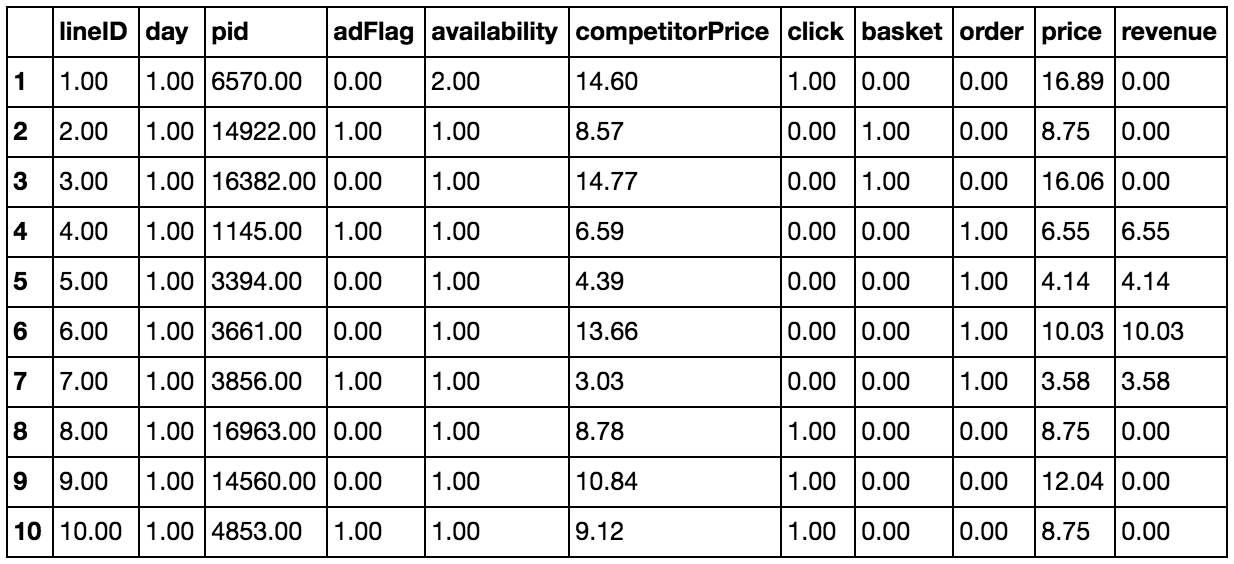
\includegraphics[scale=0.5]{graphics/dataexp.png}
	\end {figure}
\end{frame}

\begin{frame}
  \frametitle{What do the data look like?}
  \begin{block}{Training Data -- train.csv} 
    \begin{itemize}
      \item Each of 2,756,003 rows is one user action for one product
        \begin{itemize}
          \item click, basket, or order
        \end{itemize}
      \item \texttt{revenue}, a multiple of \texttt{price}
      \item Other features:
        \begin{itemize}
          \item day, adFlag, availability, price, competitorPrice
        \end{itemize}
      \item No feature to identify distinct users
    \end{itemize}
  \end{block}

  \begin{block}{Test Data -- class.csv} 
    \begin{itemize}
      \item Same structure as above, excluding user action and \texttt{revenue}
      \item 1,210,767 rows
    \end{itemize}
  \end{block}
\end{frame}

\begin{frame}
  \frametitle{What do the data look like?}
  \begin{block}{Items Data -- items.csv} 
    \begin{itemize}
      \item Each of 22,035 rows is one item
      \item Information that doesn't change over time
      \item Linked to other data sets by product ID
      \item Other features:
        \begin{itemize}
          \item manufacturer
          \item group (``product group'')
          \item content, unit
          \item pharmForm, genericProduct
          \item salesIndex (``dispensing regulation code'')
          \item category, campaignIndex
          \item rrp
        \end{itemize}
    \end{itemize}
  \end{block}
\end{frame}


\section{Exploration Results} % ----------------------------------------

\begin{frame}
  \frametitle{Initial Results}

  \begin{block}{User Actions}
  \begin{itemize}
    \item For each unique user and item, only the final action is recorded
    \item \texttt{competitorPrice} is missing for $3.7\%$ of training data
  \end{itemize}
  \end{block}

  \begin{block}{Items}
  \begin{itemize}
    \item Items with \texttt{availability} 4 rarely ordered---``out of stock''?
    \item Only $5.1\%$ of items in training data have \texttt{salesIndex} 44 or
    52
    \item 3,814 items are identical to another item, excluding ID
  \end{itemize}
  \end{block}
\end{frame}

\begin{frame}
  \frametitle{A Suspicious Pattern}

  \begin {figure}
	  \centering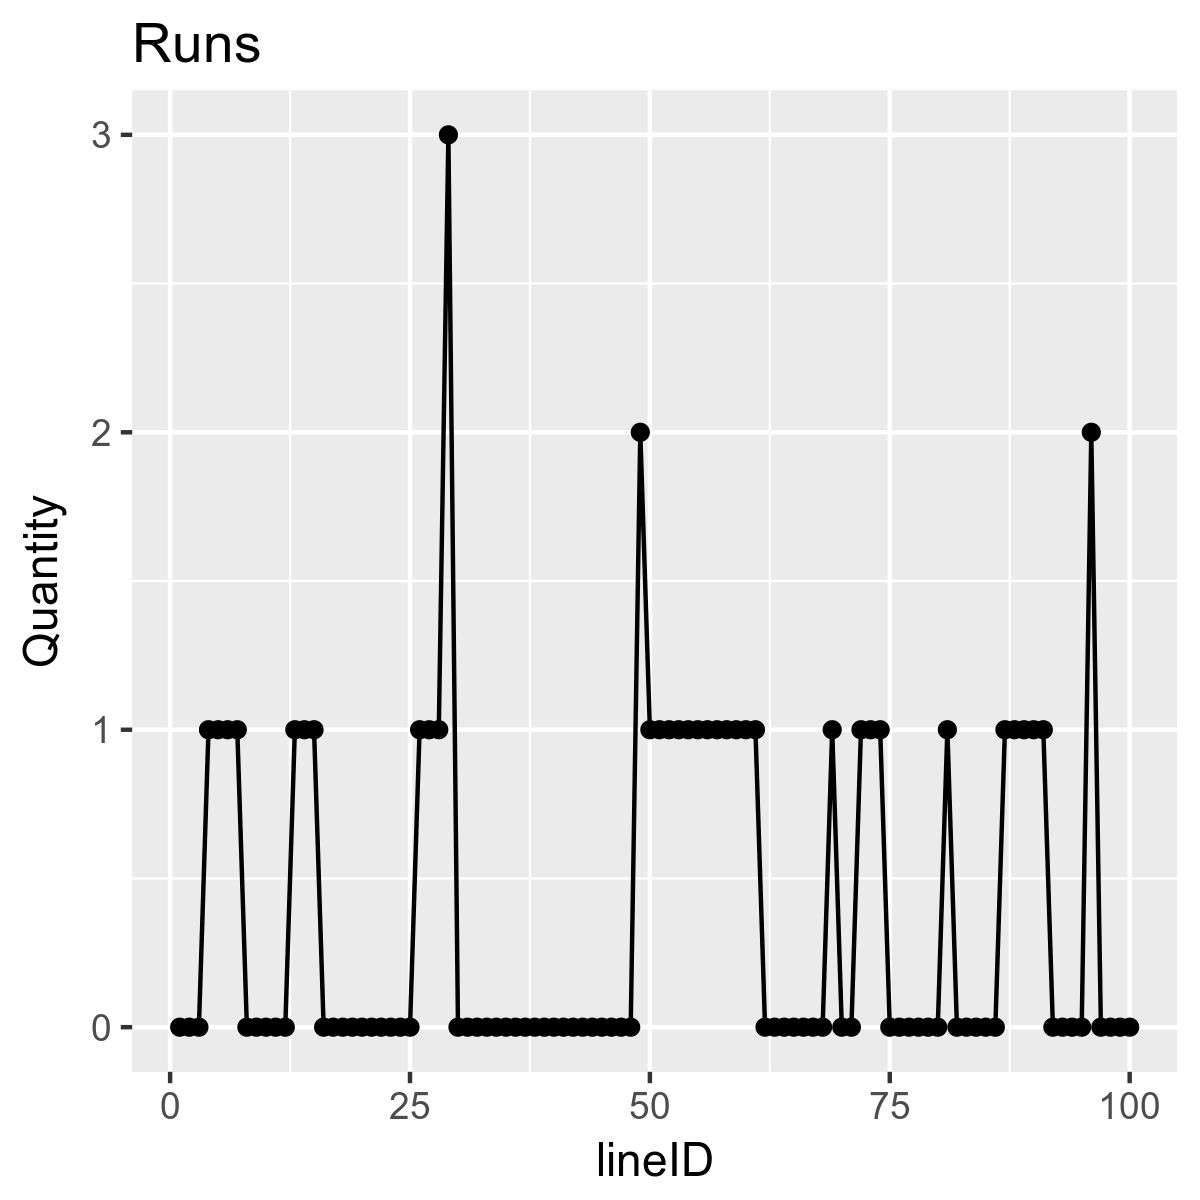
\includegraphics[scale=0.5]{graphics/runs.png}
    \quad
	  \centering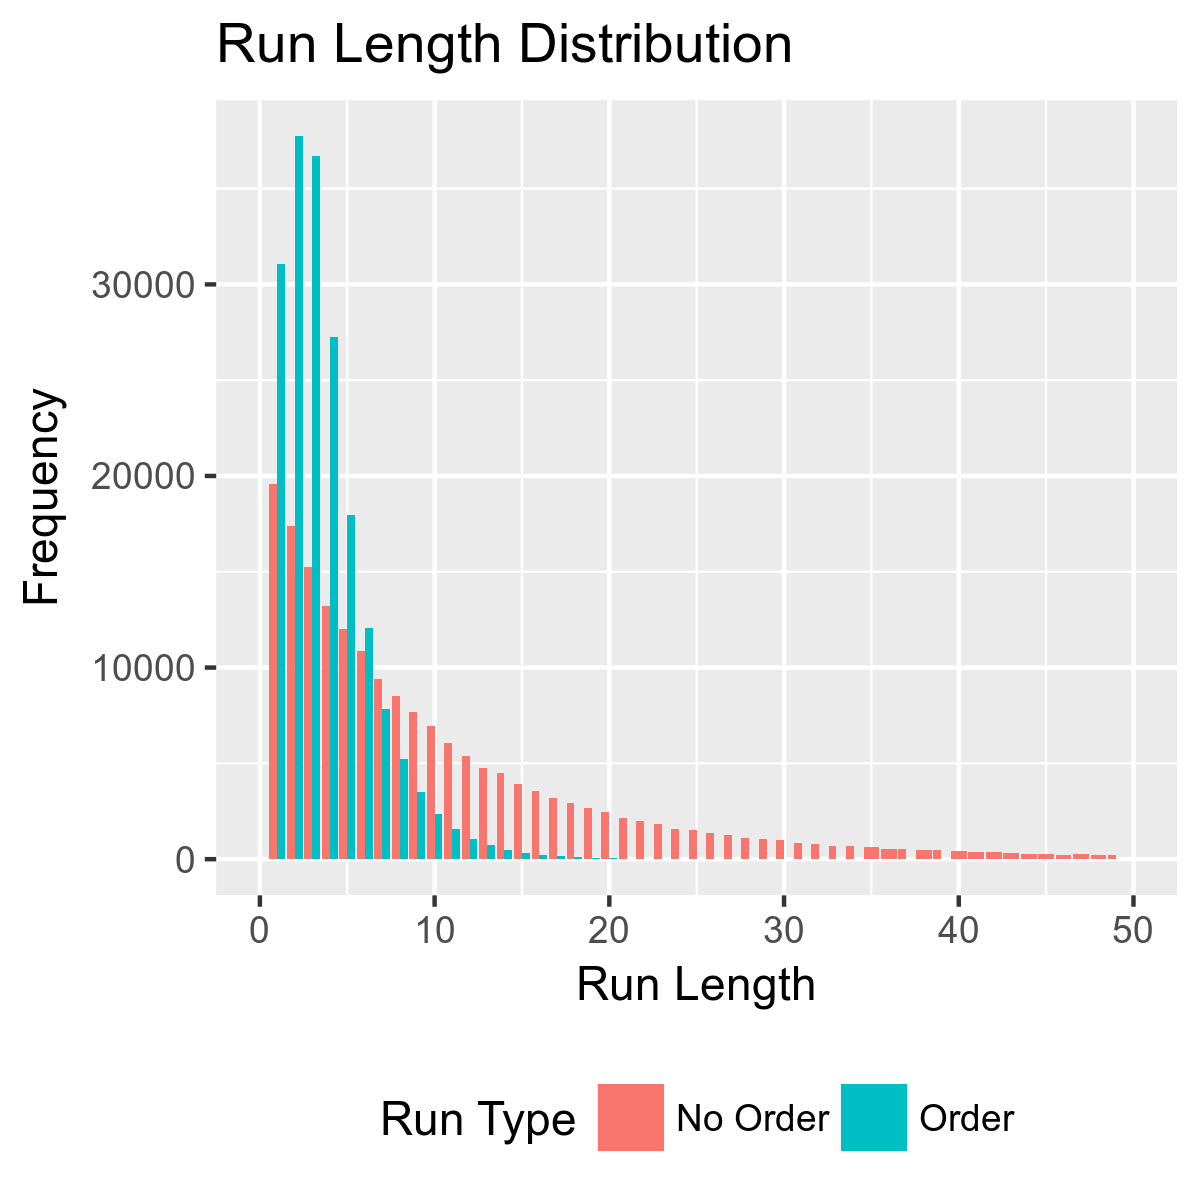
\includegraphics[scale=0.5]{graphics/run_length.png}
	\end {figure}
\end{frame}

\begin{frame}
  \frametitle{A Suspicious Pattern}

  \begin{block}{Curiouser and curiouser!}
    \begin{itemize}
    \item Runs of ``no order'' and ``order''
    \item ``No order'' run-lengths appear to have geometric distribution
    \item ``Order'' run-lengths usually less than 10
    \item Items rarely appear more than once within an ``order'' run
    \end{itemize}
  \end{block}

  \pause
  Each ``order'' run might be a single shopping basket!

\end{frame}

\begin{frame}
  \frametitle{Additional Results}
  
  \begin{block}{3-character codes in \texttt{pharmForm}}
  \begin{itemize}
    \item Example: TAB, CRE, KAP, GLO, TRO
    \item Identifies form of medicine (tablets, syrup, salve, \dots)
    \item German abbreviations, as listed on:

    \begin{itemize}
      \item \href{http://www.docmorris-blog.de/2014/8/2/medikamente-abkuerzungsverzeichnis/}{DocMorris}
      \item \href{http://www.kohlpharma.com/de/import_arzneimittel/abkuerzungen}{KohlPharma}
    \end{itemize}

    \item Closely related forms can have distinct codes
  \end{itemize}
  \end{block}
\end{frame}


\section{Feature Engineering} % ----------------------------------------

\begin{frame}
  \frametitle{Feature Engineering}
  Winning teams from many data mining competitions---including the UC Davis
  2016 DMC team---say feature engineering was the most important part of their
  strategy.
\end{frame}

\begin{frame}
  \frametitle{Planned Features}
  \begin{itemize}
    \item Day of week, day of month, week of month
    \item Windowed statistics
    \item Unit type (weight, volume, or pieces)
    \item Total units (from \texttt{content})
    \item Price per unit, \texttt{competitorPrice} per unit, \texttt{rrp} per
    unit
    \item Grouped forms (from \texttt{pharmForm})
    \item \dots
  \end{itemize}
\end{frame}

\begin{frame}
  \frametitle{Encoding Categorical Features}

  \begin{block}{One-hot encoding}
  \begin{itemize}
    \item Each category becomes a separate binary feature
    \item Models can eliminate unimportant categories
    \item Unhelpful when novel categories appear in the training data
  \end{itemize}
  \end{block}

  \begin{block}{Likelihood encoding}
  \begin{itemize}
    \item For each category, each observation is assigned a likelihood
    \begin{itemize}
      \item Likelihood is leave-one-out estimate of order probability
      \item Likelihood is 0.5 for all observations in test data
    \end{itemize}
    \item Loses information and doesn't account for order quantity
  \end{itemize}
  \end{block}
\end{frame}


\section{Potential Models} % ----------------------------------------

\begin{frame}
  \frametitle{Our Plan}
  \begin{itemize}
    \item Generate lots of features
    \item Use initial model to select important features
    \begin{itemize}
      \item Importance rankings---from random forest, for example
      \item Lasso or other regularization methods
    \end{itemize}
    \item Build an ensemble of models and refine initial model
  \end{itemize}
\end{frame}

\begin{frame}
  \frametitle{Choosing Models}
  We need advice on which models to use!

  \begin{block}{Proposed Models}
  \begin{itemize}
    \item Quantity
    \begin{itemize}
      \item Hidden (semi-)Markov model
      \item Linear-chain conditional random field
      \item Generalized linear models
      \item Boosted random forest
    \end{itemize}

    \item Revenue
  \end{itemize}
  \end{block}
\end{frame}

\begin{frame}
  \frametitle{Hidden Markov And Semi-Markov Models}
  \begin{figure}
	  \centering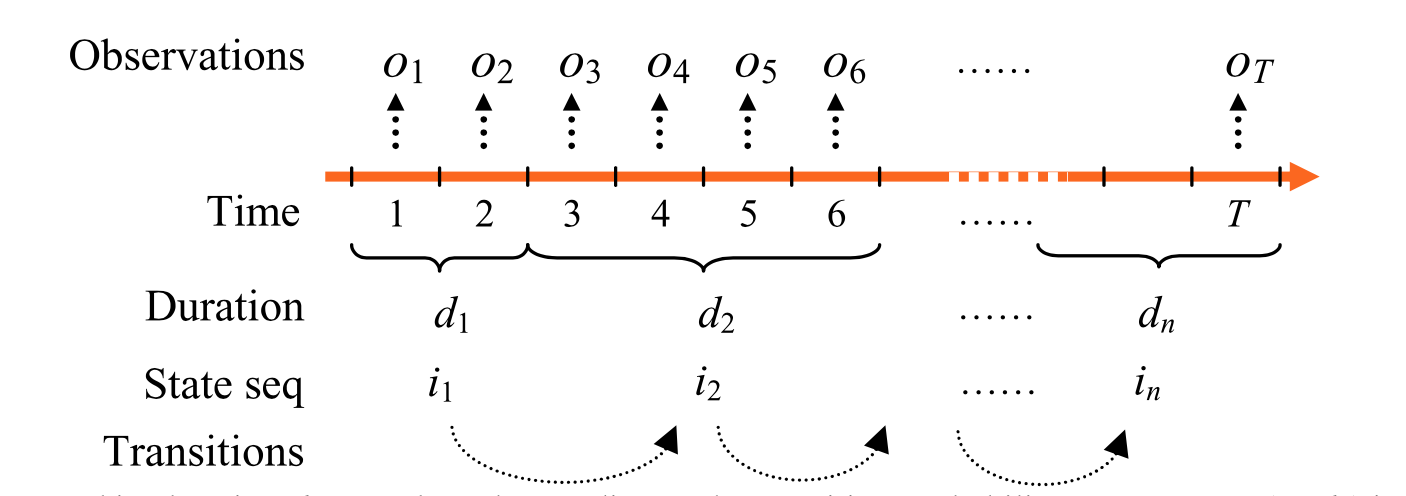
\includegraphics[scale=0.4]{graphics/semi.png}
	\end {figure}
\end{frame}

\begin{frame}
\frametitle{Hidden Markov And Semi-Markov Models}
  \begin{block}{Hidden Markov Model (HMM)}
  \begin{itemize}
    \item Each response $y_i$ comes from one of several subpopulations
    \item Subpopulations may have different distributions
    \item An unobserved Markov chain determines which subpopulation
  \end{itemize}
  \end{block}

  \begin{block}{Hidden Semi-Markov Model}
  \begin{itemize}
    \item Generalization of HMMs
    \item Time in a state can affect transition probabilities
  \end{itemize}
  \end{block}
\end{frame}

\begin{frame}
  \Huge{\centerline{Advice? Suggestions?}}
\end{frame}

\end{document} 
